\documentclass{standalone}
\usepackage{tikz}
\usetikzlibrary{patterns, positioning}

\begin{document}
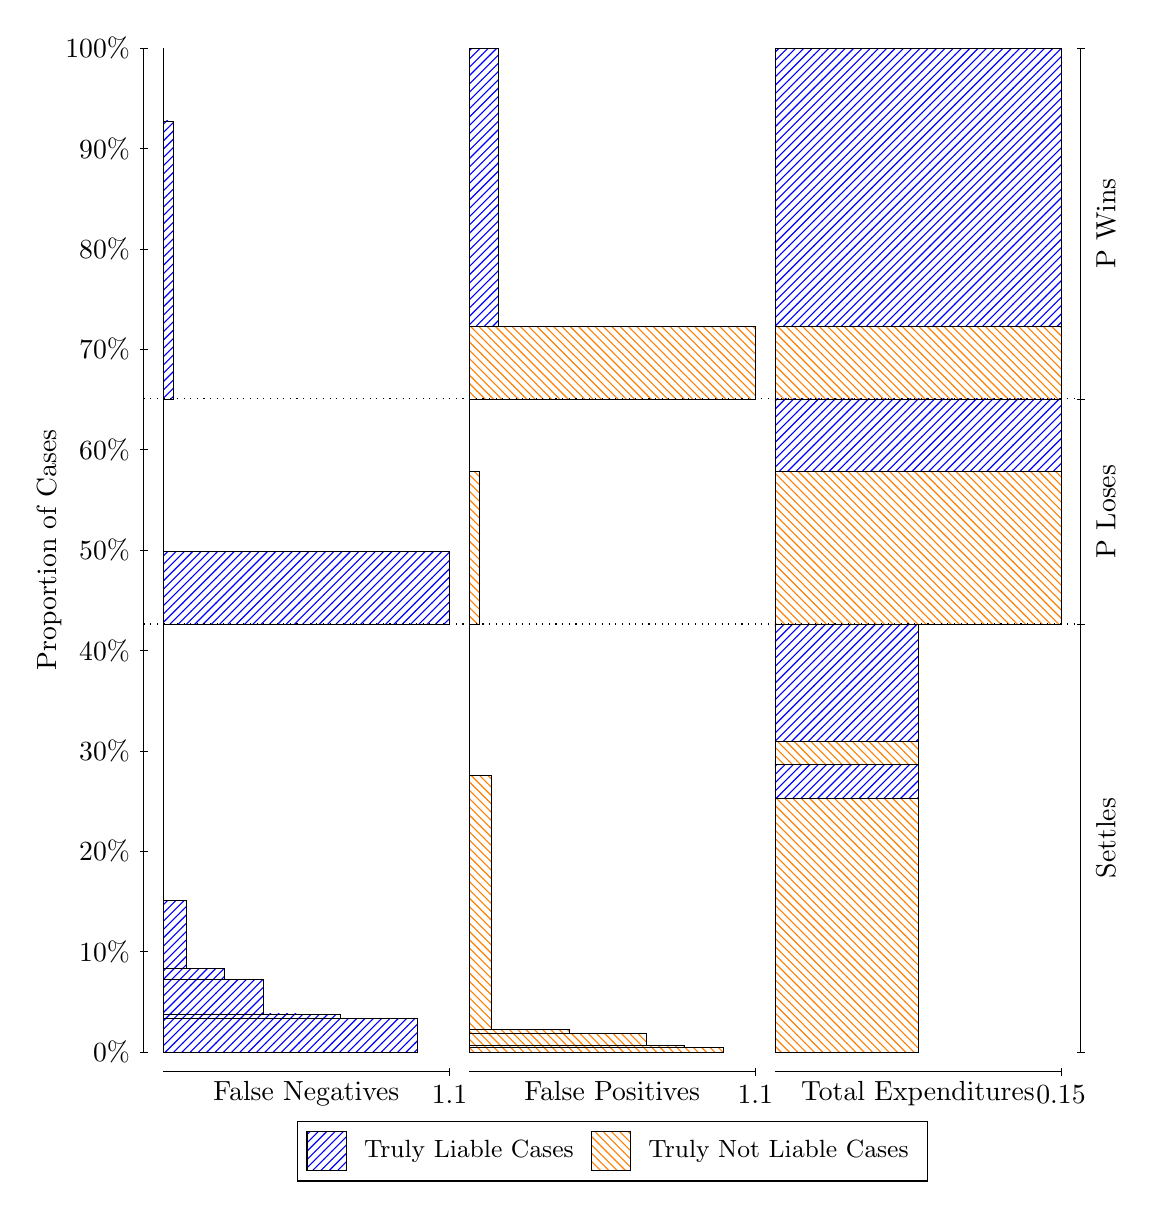
\begin{tikzpicture}
\draw[black, very thin] (1.5,1.75) -- (1.5,14.5);
\node[rotate=90, anchor=center] at (0.3, 8.125) {Proportion of Cases};
\draw[black, very thin] (1.45,1.75) -- (1.55,1.75);
\node[anchor=east] at (1.45, 1.75) {0\%};
\draw[black, very thin] (1.45,3.025) -- (1.55,3.025);
\node[anchor=east] at (1.45, 3.025) {10\%};
\draw[black, very thin] (1.45,4.3) -- (1.55,4.3);
\node[anchor=east] at (1.45, 4.3) {20\%};
\draw[black, very thin] (1.45,5.575) -- (1.55,5.575);
\node[anchor=east] at (1.45, 5.575) {30\%};
\draw[black, very thin] (1.45,6.85) -- (1.55,6.85);
\node[anchor=east] at (1.45, 6.85) {40\%};
\draw[black, very thin] (1.45,8.125) -- (1.55,8.125);
\node[anchor=east] at (1.45, 8.125) {50\%};
\draw[black, very thin] (1.45,9.4) -- (1.55,9.4);
\node[anchor=east] at (1.45, 9.4) {60\%};
\draw[black, very thin] (1.45,10.675) -- (1.55,10.675);
\node[anchor=east] at (1.45, 10.675) {70\%};
\draw[black, very thin] (1.45,11.95) -- (1.55,11.95);
\node[anchor=east] at (1.45, 11.95) {80\%};
\draw[black, very thin] (1.45,13.225) -- (1.55,13.225);
\node[anchor=east] at (1.45, 13.225) {90\%};
\draw[black, very thin] (1.45,14.5) -- (1.55,14.5);
\node[anchor=east] at (1.45, 14.5) {100\%};

\draw[black, very thin] (13.4,1.75) -- (13.4,14.5);
\draw[black, very thin] (13.35,1.75) -- (13.45,1.75);
\node[anchor=west] at (13.35, 1.75) {};
\draw[black, very thin] (13.35,7.1846) -- (13.45,7.1846);
\node[anchor=west] at (13.35, 7.1846) {};
\draw[black, very thin] (13.35,10.044) -- (13.45,10.044);
\node[anchor=west] at (13.35, 10.044) {};
\draw[black, very thin] (13.35,14.5) -- (13.45,14.5);
\node[anchor=west] at (13.35, 14.5) {};

\draw[black, very thin, pattern color=blue, pattern=north east lines] (1.75,1.75) rectangle (4.9751,2.1779);
\draw[black, very thin, pattern color=blue, pattern=north east lines] (1.75,2.1779) rectangle (3.9953,2.2253);
\draw[black, very thin, pattern color=blue, pattern=north east lines] (1.75,2.2253) rectangle (3.5054,2.2345);
\draw[black, very thin, pattern color=blue, pattern=north east lines] (1.75,2.2345) rectangle (3.0155,2.6708);
\draw[black, very thin, pattern color=blue, pattern=north east lines] (1.75,2.6708) rectangle (2.5257,2.813);
\draw[black, very thin, pattern color=blue, pattern=north east lines] (1.75,2.813) rectangle (2.0358,3.6723);
\draw[black, very thin, pattern color=orange, pattern=north west lines] (1.75,3.6723) rectangle (1.75,7.1846);
\draw[black, very thin, pattern color=blue, pattern=north east lines] (1.75,7.1846) rectangle (5.3833,8.1056);
\draw[black, very thin, pattern color=orange, pattern=north west lines] (1.75,8.1056) rectangle (1.75,10.044);
\draw[black, very thin, pattern color=blue, pattern=north east lines] (1.75,10.044) rectangle (1.8725,13.576);
\draw[black, very thin, pattern color=orange, pattern=north west lines] (1.75,13.576) rectangle (1.75,14.5);
\draw[black, very thin, pattern color=orange, pattern=north west lines] (5.6333,1.75) rectangle (8.8584,1.8086);
\draw[black, very thin, pattern color=orange, pattern=north west lines] (5.6333,1.8086) rectangle (8.3685,1.8341);
\draw[black, very thin, pattern color=orange, pattern=north west lines] (5.6333,1.8341) rectangle (7.8787,1.9849);
\draw[black, very thin, pattern color=orange, pattern=north west lines] (5.6333,1.9849) rectangle (7.3888,1.9898);
\draw[black, very thin, pattern color=orange, pattern=north west lines] (5.6333,1.9898) rectangle (6.8989,2.0414);
\draw[black, very thin, pattern color=orange, pattern=north west lines] (5.6333,2.0414) rectangle (5.9191,5.2623);
\draw[black, very thin, pattern color=blue, pattern=north east lines] (5.6333,5.2623) rectangle (5.6333,7.1846);
\draw[black, very thin, pattern color=orange, pattern=north west lines] (5.6333,7.1846) rectangle (5.7558,9.1233);
\draw[black, very thin, pattern color=blue, pattern=north east lines] (5.6333,9.1233) rectangle (5.6333,10.044);
\draw[black, very thin, pattern color=orange, pattern=north west lines] (5.6333,10.044) rectangle (9.2667,10.968);
\draw[black, very thin, pattern color=blue, pattern=north east lines] (5.6333,10.968) rectangle (6.0007,14.5);
\draw[black, very thin, pattern color=orange, pattern=north west lines] (9.5167,1.75) rectangle (11.333,4.9709);
\draw[black, very thin, pattern color=blue, pattern=north east lines] (9.5167,4.9709) rectangle (11.333,5.3988);
\draw[black, very thin, pattern color=orange, pattern=north west lines] (9.5167,5.3988) rectangle (11.333,5.6902);
\draw[black, very thin, pattern color=blue, pattern=north east lines] (9.5167,5.6902) rectangle (11.333,7.1846);
\draw[black, very thin, pattern color=orange, pattern=north west lines] (9.5167,7.1846) rectangle (13.15,9.1233);
\draw[black, very thin, pattern color=blue, pattern=north east lines] (9.5167,9.1233) rectangle (13.15,10.044);
\draw[black, very thin, pattern color=orange, pattern=north west lines] (9.5167,10.044) rectangle (13.15,10.968);
\draw[black, very thin, pattern color=blue, pattern=north east lines] (9.5167,10.968) rectangle (13.15,14.5);
\draw[black, dotted] (1.5,7.1846) -- (13.4,7.1846);
\draw[black, dotted] (1.5,10.044) -- (13.4,10.044);
\draw[black, very thin] (1.75,1.5) -- (5.3833,1.5);
\node[anchor=north] at (3.5667, 1.5) {False Negatives};
\draw[black, very thin] (5.3833,1.45) -- (5.3833,1.55);
\node[anchor=north] at (5.3833, 1.45) {1.1};

\draw[black, very thin] (5.6333,1.5) -- (9.2667,1.5);
\node[anchor=north] at (7.45, 1.5) {False Positives};
\draw[black, very thin] (9.2667,1.45) -- (9.2667,1.55);
\node[anchor=north] at (9.2667, 1.45) {1.1};

\draw[black, very thin] (9.5167,1.5) -- (13.15,1.5);
\node[anchor=north] at (11.333, 1.5) {Total Expenditures};
\draw[black, very thin] (13.15,1.45) -- (13.15,1.55);
\node[anchor=north] at (13.15, 1.45) {0.15};

\node[black, centered, rotate=90] at (13.72, 4.4673) {Settles};
\node[black, centered, rotate=90] at (13.72, 8.6144) {P Loses};
\node[black, centered, rotate=90] at (13.72, 12.272) {P Wins};

\draw (7.449999999999999,1.5) node[draw=none] (baseCoordinate) {};
\begin{scope}[align=center]
        \matrix[scale=0.5, draw=black, below=0.5cm of baseCoordinate, nodes={draw}, column sep=0.1cm]{
            \node[rectangle, draw, minimum width=0.5cm, minimum height=0.5cm, pattern=north east lines, pattern color=blue] {}; &
            \node[draw=none, font=\small] (B) {Truly Liable Cases}; &
            \node[rectangle, draw, minimum width=0.5cm, minimum height=0.5cm, pattern=north west lines, pattern color=orange] {}; &
            \node[draw=none, font=\small] (B) {Truly Not Liable Cases}; \\
            };
\end{scope}

\end{tikzpicture}
\end{document}